\S4.1--4.2 are analytical (template game); the rest use 200 seeds per configuration, the same for every policy.
Unless stated, Red plays MIP-BR with $\varepsilon_\Rd=0.15$ in nominal weather.

\subsection{Small example: patrol or assert, and sustainable restraint}
Fix the force splits that survive dominance (\S4.2): Blue center-heavy, Red south-heavy. Each side then only
chooses P or A. The resulting $2\times2$ sub-matrix of $\Gamma$, normalized so (P,P) $=(0,0)$, has
(P,A) $=(-9.61,\,1.20)$, (A,P) $=(0.28,\,-10.45)$ and (A,A) $=(-11.41,\,-11.33)$ (Blue, Red).
Asserting against a patroller pays a little (one-period gain $G_\B=0.28$, $G_\Rd=1.20$), but mutual assertion costs more than
patrolling alone, so $BR_i(\Pt)=\As$ and $BR_i(\As)=\Pt$: the same structure as the
shared-compute example (Lecture 3). There are two pure NE, (A,P) and (P,A), and a mixed NE (Blue asserts w.p.\
$0.58$, Red $0.13$) with mutual assertion w.p.\ $0.08$ and payoffs $v_\B=-1.25$, $v_\Rd=-6.06$. The welfare-maximizing correlated equilibrium (CE LP)
puts $0.40$ on (P,P), $0.54$ on (A,P), $0.06$ on (P,A) and \emph{zero} on (A,A): a mediator (e.g.\ a hotline)
removes mutual assertion.

In the repeated game (Lectures 5--6), consider grim trigger: both patrol; after any assertion, both play the
mixed NE forever. By the one-stage deviation principle, patrolling is optimal iff
$(1-\delta)G_i+\delta v_i\le0$, i.e.\ $\delta\ge G_i/(G_i-v_i)$, which is $0.18$ for Blue and $0.17$ for Red. With
$\delta=0.98$, \textbf{mutual restraint is a subgame perfect equilibrium}, although our one-period-ahead policies
cannot see this yet.

\subsection{Template game: dominance, equilibria and the effect of the escalation cost}
IESDS reduces $\Gamma$ from $14\times14$ to $2\times4$: Blue keeps only the center-heavy split (20\% North, 60\% Center, 20\% South),
Red the south- or center/south-heavy splits. There are two pure NE: (Blue C-heavy assert, Red S-heavy patrol),
payoffs $(0.39,-9.27)$, and (Blue C-heavy patrol, Red C/S assert), $(-14.44,2.71)$; the \emph{equilibrium} policy
plays the first (higher total payoff; this selection is an assumption). Without the escalation cost, the zero-sum
maximin LP has a pure equilibrium where \emph{both} sides concentrate on the Center and assert (value $-2.26$):
the shared incident cost is what makes at most one side assert.

\subsection{RQ1: control versus war risk, and the risk-budget game}
\begin{figure}[!ht]
\centering
\begin{minipage}{0.40\textwidth}\centering
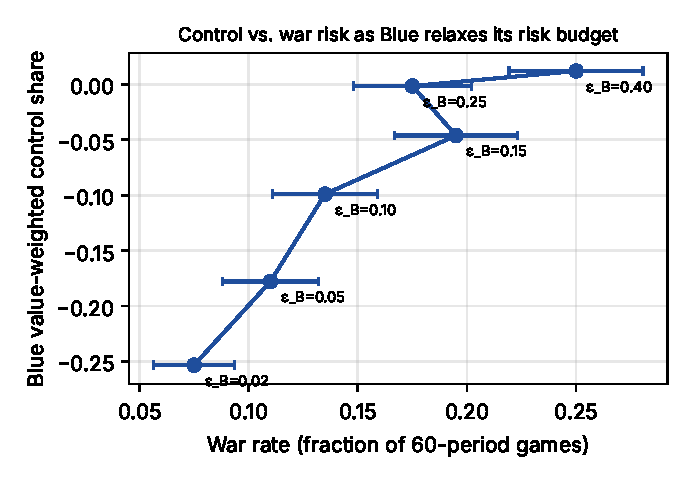
\includegraphics[width=\textwidth,height=3.7cm,keepaspectratio]{figures/frontier.pdf}
\end{minipage}\hfill
\begin{minipage}{0.54\textwidth}\centering\small
\begin{tabular}{l|ccc}
\toprule
$\B\backslash\Rd$ & cons.\ $0.05$ & mod.\ $0.15$ & aggr.\ $0.40$\\\midrule
cons.\ $0.05$ & $-194,\ 199$ & $-303,\ 315$ & $-308,\ 318$\\
              & war $0.10$ & $0.11$ & $0.12$\\
mod.\ $0.15$  & $18,\ -36$ & $-144,\ 101$ & $-192,\ 140$\\
              & war $0.15$ & $0.20$ & $0.21$\\
aggr.\ $0.40$ & $74,\ -80$ & $-83,\ 16$ & $\mathbf{-151,\ 39}$\\
              & war $0.14$ & $0.25$ & $\mathbf{0.34}$\\
\bottomrule
\end{tabular}
\end{minipage}
\caption{Left: Blue's control share vs.\ war rate as Blue's risk budget $\varepsilon_\B$ grows (Red fixed at $0.15$).
Right: the risk-budget game, $(u_\B,u_\Rd)$ and war rate when both sides choose $\varepsilon$ (s.e.\ $\approx 5$--$12$).
Bold: the unique Nash equilibrium.}
\label{fig:rq1}
\end{figure}
\textbf{Frontier.} Raising $\varepsilon_\B$ from $0.02$ to $0.15$ lifts Blue's control share from $-0.25$ to
$-0.05$ while the war rate rises from $0.07$ to $0.20$; going to $0.40$ adds only $0.06$ of control
(Fig.~\ref{fig:rq1}). Most of what a looser budget buys is bought by $\varepsilon\approx0.15$--$0.25$.

\textbf{Risk-budget game.} When both sides pick a budget, ``aggressive'' is a best response to every opponent
choice for both players (Red vs.\ conservative Blue, $318$ vs.\ $315$, is within noise), so (aggressive,
aggressive) is the unique pure NE. It has the \emph{highest} war rate ($0.34$ vs.\ $0.10$ when both are
conservative) and total payoff $-112$ vs.\ $+12$ at (conservative, moderate): a prisoner's dilemma (Lecture 3).
So restraint must come from repetition or coordination (\S4.1).

\subsection{RQ2: strategic versus heuristic play}
\begin{table}[!ht]\centering\small
\begin{tabular}{l|ccc|c}
\toprule
Blue $\backslash$ Red & rule-based (moderate) & MIP-BR & equilibrium & worst case over Red\\\midrule
random & $-283$ / $-0.14$ / $0.15$ & $-319$ / $-0.16$ / $0.33$ & $-164$ / $-0.08$ / $0.06$ & $-319$\\
rule-based (moderate) & $-122$ / $-0.05$ / $0.04$ & $-184$ / $-0.09$ / $0.06$ & $35$ / $+0.06$ / $0.04$ & $-184$\\
greedy & $-70$ / $+0.01$ / $0.12$ & $-137$ / $-0.05$ / $0.14$ & $65$ / $+0.08$ / $0.03$ & $-137$\\
MIP-BR & $-75$ / $+0.01$ / $0.13$ & $-144$ / $-0.05$ / $0.20$ & $53$ / $+0.08$ / $0.08$ & $-144$\\
equilibrium & $-72$ / $-0.01$ / $0.07$ & $\mathbf{-116}$ / $-0.03$ / $0.10$ & $21$ / $+0.05$ / $0.06$ & $\mathbf{-116}$\\
maximin & $-170$ / $-0.09$ / $0.04$ & $-221$ / $-0.12$ / $0.08$ & $-35$ / $-0.01$ / $0.00$ & $-221$\\
\bottomrule
\end{tabular}
\caption{Blue payoff $u_\B$ / control share / war rate (s.e.\ of $u_\B$ is 1--7). Nominal weather, design D0.}
\label{tab:policies}
\end{table}
Greedy, MIP-BR and equilibrium beat the random and rule-based benchmarks (Table~\ref{tab:policies}). The
\textbf{equilibrium} policy has the best worst case over Red's policies ($-116$) and, against MIP-BR, half the war
rate of MIP-BR itself ($0.10$ vs.\ $0.20$). Greedy and MIP-BR do best against weaker opponents but escalate more.
\textbf{Maximin} is the safest (war rate $\le0.08$) but gives up the most control: it guards against a worst-case
Red template that Red rarely plays.

\textbf{MIP vs.\ greedy.} Over 1{,}524 Blue decisions in 30 games the greedy heuristic matched the MIP optimum
in 67\% of decisions but broke the risk budget in 14\%, so the MIP is needed to enforce the feasible region
exactly; in play the two perform about the same.

\subsection{RQ3: robustness to weather and resilient designs}
\subsection{RQ3: weather robustness and resilient designs}
For policy or design $x$, let $J(x,\omega)$ be its simulated mean payoff under scenario $\omega$.
We compare $\sum_\omega\pi_\omega J(x,\omega)$ and $\min_\omega J(x,\omega)$.
The latter is the worst scenario mean, not the worst individual run or worst possible opponent.
\begin{figure}[H]\centering
\begin{minipage}{0.35\textwidth}\centering
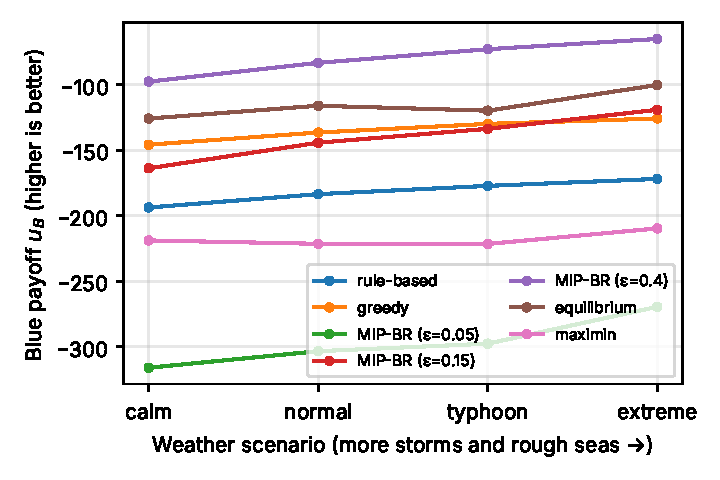
\includegraphics[width=\textwidth]{figures/weather.pdf}
\end{minipage}\hfill
\begin{minipage}{0.63\textwidth}\centering\small
\setlength{\tabcolsep}{3pt}
\begin{tabular}{@{}lrrrrrr@{}}\toprule
Design & Calm & Nom. & Typh. & Extr. & Exp. & Worst\\\midrule
D0 & $-164$ & $-144$ & $-134$ & $-119$ & $-144$ & $-164$\\
D1 & $-153$ & $-141$ & $-131$ & $\mathbf{-98}$ & $-137$ & $-153$\\
D2 & $-181$ & $-164$ & $-149$ & $-136$ & $-162$ & $-181$\\
D3 & $\mathbf{-140}$ & $\mathbf{-118}$ & $\mathbf{-111}$ & $-102$ & $\mathbf{-120}$ & $\mathbf{-140}$\\\bottomrule
\end{tabular}
\end{minipage}
\caption{Left: Blue policy payoffs by weather. Right: Blue design payoffs with MIP-BR on both sides
(reported s.e.\ approximately 7); D0 baseline, D1 basing, D2 sensing, D3 hotline.}\label{fig:rq3}
\end{figure}
\textbf{Weather.} Most tested policies do worst in calm seas: rough seas weaken Red's CCG hulls and storms
pause incidents. Baseline MIP-BR's war rate falls from $0.24$ (calm) to $0.10$ (extreme). MIP-BR with
$\varepsilon_\B=0.40$ and the equilibrium-derived policy rank first and second in all four scenarios.
The highest-payoff policy also has war rates of $0.12$--$0.29$, making sensitivity to $W=200$ important.

\textbf{Designs.} D3 has the best expected and worst-scenario payoff; in nominal weather it cuts war rate
from $0.20$ to $0.05$ and increases Red's payoff from $101$ to $144$. Its zero cost is an assumption.
D1 barely changes Blue's nominal payoff, reduces Red's from $101$ to $16$, and raises war rate to $0.28$.
D2 shows no measurable benefit even in the reported zero-cost check. Red recomputes actions under its
fixed MIP-BR policy; these experiments do not re-solve equilibrium policy selection after redesign.

\textbf{Limits of inference.} Numerical values are assumptions. The findings are comparisons within the model,
not calibrated forecasts of conflict. War rates depend on hazards, de-escalation and war penalties.
Small payoff gaps should be treated cautiously given Monte Carlo error; formal comparisons require
uncertainty estimates for payoff differences. The engine's return-move cap can also make executed positions
differ from the MIP's prescribed fixed positions when returns alone exceed the cap.


\textbf{Limitations.} Parameters are assumptions; policies look one period ahead; the war rate depends strongly on
$h$, $\mu$ and $W$; payoff differences below about 20 are ties (s.e.\ 5--12).
